% !TeX root = AstCreator.tex
\definecolor{dkgreen}{rgb}{0,0.6,0}
\definecolor{gray}{rgb}{0.5,0.5,0.5}
\definecolor{mauve}{rgb}{0.58,0,0.82}
\lstnewenvironment{astlst}[1][]%
{\lstset{basicstyle=\footnotesize\ttfamily,language=Java, morekeywords={Packages,Tokens,Abstract,Syntax,Tree,Aspect,Declaration},frame=single,stringstyle=\color{mauve},commentstyle=\color{dkgreen}}#1}
{}



\section{Syntax}

The new AST that has been developed has an improved structure compared to both the existing Overture and VDMJ trees. The main addition made here is the ability to extend an AST while keeping the changes isolated in a plug-in architecture, explained in detail in section~\ref{sec:astExtendIsolation}. Secondly, the AST is specified using a grammar file inspired by SableCC\footnote{\url{http://www.sablecc.org/}}, and can generated to both VDM and Java as supported by \texttt{ASTGen}. The main structural change compared to the Overture AST is the ability to add fields to super classes.








The syntax is divided into a number of sections:

\begin{description}

\item[\textbf{\texttt{Packages}}] This section allowed the default packages to be defined for \texttt{base} that forms the basis for all nodes if nothing else is specified and \texttt{analysis} where all visitors will be generated under:

\begin{astlst}
Packages
base org.overture.ast.node;
analysis org.overture.ast.analysis;
\end{astlst}


\begin{figure}[h]

  \centering
    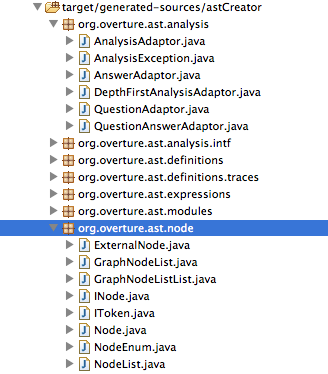
\includegraphics[width=0.5\textwidth]{figures/packageOutput}
      \caption{The package structure of the generated example.}
\end{figure}

\item[\textbf{\texttt{Tokens}}] This section defines tokens or external nodes that can be used as fields in the AST. \textit{The important part here is that they must be clonable}. Tokens  are non-generated classes which are used by the generated nodes. Tokens can be used as fields of AST Nodes and are Java classes. The following types of tokens can be specified:
\begin{description}
\item [Token] A token is an instance of the class \texttt{Token}, it is automatically generated from a name plus the text it represents.

\item [Standard Java Types] Standard Java types (basic types) can be used in the class form. These tokens start with the keyword \texttt{java:}. The use of those relies on them being passed by value when cloning is done. E.g. \texttt{Integer, Boolean, Long, Character, ...}

\item [External Java enum] This is like the standard Java type where the type given is a Java \texttt{enum}.  These tokens start with the keyword \texttt{java:enum:}

\item [External classes] Any external class can be used as a field in the AST but it must implement the interface \texttt{ExternalNode} that provides a handle to the AST for proper cloning for the node.  These tokens start with the keyword \texttt{java:}

\item [External defined Node] This enables a node to be specified outside the AST creator but still included in the analysis. The class must extend \texttt{Node} and do a proper implementation of the analysis methods and kind methods returning the correct enumeration.  These tokens start with the keyword \texttt{java:node:}

\end{description}

\begin{astlst}
Tokens
//Token 
bool = 'bool'; 
//Standard Java Type
java_Integer = 'java:java.lang.Integer'; 
//External Java enum
nameScope = 'java:enum:org.overturetool.vdmj.typechecker.NameScope';
//External Java type
location = 'java:org.overturetool.vdmj.lex.LexLocation'; 
//External defined node
LexToken = 'java:node:org.overturetool.vdmj.lex.LexToken'; 
\end{astlst}

\item[\texttt{Abstract Syntax Tree}] This section describes the tree. Names at the top level are considered roots and \# are considered sub roots. Sub roots must be  specified as a root and a child. 

\begin{astlst}
Abstract Syntax Tree
exp {-> package='org.overture.ast.expressions'}
    =   {binary} [left]:exp [op]:binop [right]:exp
    |   ...
    ;

binop {-> package='org.overture.ast.expressions'}
    = {and}
    |   {or}
    |   ...
    ;
\end{astlst}


%#Unary {-> package='org.overture.ast.expressions'}
%    =   {absolute} 
%    |   {head} 
%    |   {mapInverse} (mapType):type.#Map
%    ;

The above example will generate a tree like:
\begin{figure}[htb]
\begin{minipage}{0.5\linewidth}

\texttt{
\Tree[.exp [.binary left:exp op:binop right:exp ] ]}
\caption{AST Example.}

\end{minipage}
\begin{minipage}{0.5\linewidth}

\texttt{
\Tree[.PExp [.ABinaryExp left:PExp op:PBinop right:PExp ] ]}
\caption{AST Java Generated code Example.}

\end{minipage}
\end{figure}

\begin{description}
\item [The type of field]:
Fields can be specified in two different ways:
\begin{description}
\item[Tree]: Tree fields are fields that belong to a single node in tree and only that one. A tree node cannot be a child of any other node in the tree. Thus if an instance is assigned to a tree field the parent it may belong to is disconnected such that the child/parent relation ship is preserved.\\
Tree fields are syntactically specified as: \texttt{[feld]:type}, where \texttt{field} is the name and \texttt{type} is the type name.
\item[Graph]: Graph fields are reference fields thus the get parent will not deterministically return a single parent but just the first parent the instance was added as a reference field of. This type of node can e.g. be used to add type information to nodes where the type is a reference to a shared type. \\
Tree fields are syntactically specified as: \texttt{(field):type}, where \texttt{field} is the name and \texttt{type} is the type name.
\end{description}

\item [Field types]:
Fields must define the type of the field as a name reference to a tree element like shown in listing~\ref{} above. The syntax is \texttt{:type} where the type can be any of the below shown references:
\begin{description}
\item[Simple types]: Simple types is just the type name like \texttt{:exp} or if a nested type is given \texttt{exp.\#unary.abs}
\item[Lists]: Lists are specified as simple types but appended with a star \texttt{:exp*}
\item[Double lists]: List simple types but with two stars \texttt{:exp**}
\end{description}

\item [Sub-classing]: A sub class can be made by specifying a root as an alternative of another root. The naming convention dictates that the sub class roots must begin with \#. See Figures \ref{fig:ASTExample} and \ref{fig:ASTJavaExample}


\begin{figure}[htb]
\begin{minipage}{0.5\linewidth}

\texttt{
\Tree[.exp \#unary ]}
\\
and
\\

\texttt{
\Tree[.\#unary abs minus ]}
\caption{AST Example.}
\label{fig:ASTExample}
\end{minipage}
\begin{minipage}{0.5\linewidth}

\texttt{
\Tree[.PExp [.SUnaryExp AAbsUnaryExp AMinusUnaryExp ] ]}
\caption{AST Java Generated code Example.}
\label{fig:ASTJavaExample}
\end{minipage}
\end{figure}

\end{description}

\item[\textbf{\texttt{Aspect Declaration}}] This is a feature that allows any fields to be added to base classes (root classes in the AST grammar, the nodes where a a package can be specified). One example could be to add a \texttt{location} field to all nodes of the \texttt{exp} type. The field will be the first declared field in any of the sub classes of \texttt{exp}. The syntax looks like this:

\begin{astlst}
Abstract Declaration
%exp = [location]:location
    ;
\end{astlst}
Where \% prefixes the root node name. The name can also be a composite name like \texttt{\%exp.\#unary}.

\end{description}

\section{Node's ``toString"}

The toString macro-processing enables nodes to have a custom toString to make debugging easier. The  AST is generated with a toString function that prints all fields one after another. However, in some cases debugging might be eased by printing the node in a more suitable format (e.g. in the syntax of the language at hand). To allow such customization a macro-processor is available together with a small language.

The base princiles is that all fields of a node is accessed as defined in the AST e.g. field 1 is accessed through [field1] and strings can be added around the fields by a quoted test ''example test''. The custom toString is defined per node by \%node->sub1 = and can only be defined for leafs of the tree (\textbf{A}-nodes). Furthermore, it is possible to embed java withing the toString by using \$ to escape to java. If external java classes are to be used withing the toString any imports that might be used must be specified in the begining of the file with the \texttt{\textbf{import}} keyword as shown below:

\begin{lstlisting}[language=java,tabsize=2,basicstyle=\ttfamily\footnotesize]
To String Extensions
// import packages used by external $$ java code
import org.overture.ast.util.Utils;
import org.overture.ast.util.ToStringUtil;


//  Expressions

%exp->apply = [root] "(" + $Utils.listToString($ [args] $)$ + ")"
\end{lstlisting}


